% !TEX TS-program = pdflatex
% !TEX encoding = UTF-8 Unicode

% This is a simple template for a LaTeX document using the "article" class.
% See "book", "report", "letter" for other types of document.

\documentclass[11pt]{article} % use larger type; default would be 10pt

\usepackage[utf8]{inputenc} % set input encoding (not needed with XeLaTeX)

%%% Examples of Article customizations
% These packages are optional, depending whether you want the features they provide.
% See the LaTeX Companion or other references for full information.

%%% PAGE DIMENSIONS
\usepackage{geometry} % to change the page dimensions
\geometry{a4paper} % or letterpaper (US) or a5paper or....
% \geometry{margin=2in} % for example, change the margins to 2 inches all round
% \geometry{landscape} % set up the page for landscape
%   read geometry.pdf for detailed page layout information

\usepackage{graphicx} % support the \includegraphics command and options

% \usepackage[parfill]{parskip} % Activate to begin paragraphs with an empty line rather than an indent

%%% PACKAGES
\usepackage{booktabs} % for much better looking tables
\usepackage{array} % for better arrays (eg matrices) in maths
\usepackage{paralist} % very flexible & customisable lists (eg. enumerate/itemize, etc.)
\usepackage{verbatim} % adds environment for commenting out blocks of text & for better verbatim
\usepackage{subfig} % make it possible to include more than one captioned figure/table in a single float
\usepackage{hyperref}
\hypersetup{colorlinks=true,linkcolor=black,filecolor=magenta,urlcolor=cyan}
\usepackage{amsmath}
% These packages are all incorporated in the memoir class to one degree or another...

%%% HEADERS & FOOTERS
\usepackage{fancyhdr} % This should be set AFTER setting up the page geometry
\pagestyle{fancy} % options: empty , plain , fancy
\renewcommand{\headrulewidth}{0pt} % customise the layout...
\lhead{}\chead{}\rhead{}
\lfoot{}\cfoot{\thepage}\rfoot{}

%%% SECTION TITLE APPEARANCE
\usepackage{sectsty}
\allsectionsfont{\sffamily\mdseries\upshape} % (See the fntguide.pdf for font help)
% (This matches ConTeXt defaults)

%%% ToC (table of contents) APPEARANCE
\usepackage[nottoc,notlof,notlot]{tocbibind} % Put the bibliography in the ToC
\usepackage[titles,subfigure]{tocloft} % Alter the style of the Table of Contents
\renewcommand{\cftsecfont}{\rmfamily\mdseries\upshape}
\renewcommand{\cftsecpagefont}{\rmfamily\mdseries\upshape} % No bold!

%%% END Article customizations

%%% The "real" document content comes below...

\title{sptPALM Analysis Guide}
\author{Adam Hines}
\date{}

\begin{document}
\maketitle

%%% Table of Contents Section %%%%
\newpage
\tableofcontents

\newpage

\section{Introduction}

Thank you for downloading and trying sptPALM Analysis (SPA). SPA is a semi-automated single particle tracking tool utilising a graphical user interface (GUI) that interfaces with the ImageJ plugin TrackMate. Users are able to automatically load image sequences of photoactivatable localisation microscopy (PALM) and utilise a built in tracking algorithm for single particles (spt). The semi-automated component refers to the fact that users are required to convert image sequences to the correct format and determine threshold values for spot detection themselves. This is advantageous as auto-detecting threshold values can often lead to over or under-estimation of the spot detection threshold. \\
SPA was developed by Adam Hines at the Queensland Brain Institute. If utilising this tool in your publications, please cite (\textit{reference}) as well as the original author of TrackMate (\textit{reference}).

\subsection{Overview}

This chapter will provide an overview on how the analysis script operates and what algorithms the program uses in order to reliably detect and track the mobility of particles. It will begin by briefly describing the spot detection component of the analysis and the tracking algorithm utilised, however for further information please refer to the source documentation of TrackMate (\href{https://imagej.net/TrackMate_Algorithms}{TrackMate Algorithms}).

\subsection{Spot detection}

The chosen method for spot detection was the Lapacian of Gaussian (LoG) fitting algorithm. This algorithm takes low resolution spots and fits a LoG over pixels in an x,y plane. The threshold specified will determine which detected spots are appropriate and which are not, and this should be done by the user with their own eyes as this avoids having too many innappropriate or too few appropriate spots. A visualisation of how the spot detection algorithm works is presented in Figure 1.\\

There are also two settings that are enabled during the spot detection component of SPA. Median filtering and subpixel localisation are enabled to remove the generation of 'jagged' particle linked tracks as well as to improve the acuity of spot detection.\\

There are other methods for spot detection available in TrackMate, and it should be encouraged to explore the best option for your needs. Embedded into the software however is the LoG detection. SPA is an open-sourced program, so editing the source code will be your only option in order to hardwire a difference detection algorithm - and the same goes for the tracking method (covered in the next section).

	\begin{figure}
	\center{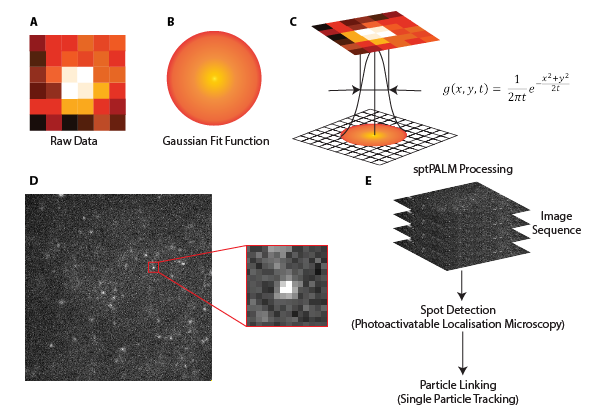
\includegraphics[width=\textwidth]{Figures/"1) Introduction"/PALM-01.png}}
	\caption{Visualisation of particle detection in SPA. \textbf{A} Schematic of typical raw data observed in photoactivatable light microscopy (PALM) 					experiments, consisting of low resolution pixels with a bright centre with decreasing intensity from the centre. \textbf{B} Example of a Gaussian fit of the raw 		data in \textbf{A}. \textbf{C} The Gaussian fit function transposing the low resolution raw data into a high-resolution spot. Formula shown if the Lapacian of 		Gaussian (LoG) spot detection used in SPA analysis. \textbf{D} Representative raw data from a PALM experiment highlighting a single spot. \textbf{E} 				Schematic of the workflow used in SPA. Image sequences have parallel threading in spot detection and particle linking in subsequent tracking stages of 			analysis.}
	\end{figure}

\subsection{Particle linking}

Single particle tracking has remained a problem for researchers for a very long time. Reliable tracking of multiple particles over a long time frame can cause issues such as linking particles together that are not the same, incorrectly linking a particle that has newly appeared, or even incorrectly ending a track. Figure 2 \textbf{A} shows an example of what a tracked particle looks like in an x,y plane. SPA uses the particle linking algorithm known as a linear assignment problem (LAP) cost matrix in order to evaluate and ultimately minimise the cost in favour of the most likely linked particles between frame  $t_1$ and $t_2$. The cost values in this context is simply the squared displacement ($\delta^2$) between two detected particles. Each particle in frame $n_1$ has a potential link associated to every particle in frame $t_2$ (Figure 2 \textbf{B}), meaning that for each particle in $t_1$ there are several cost values associated to that particle and the LAP algorithm attempts to find the lowest sum cost for every single particle between frames $t_1$ and $t_2$. \\

What about particles that have no prior or future link? At a certain point during a recording, particles will bleach and new particles will appear, so how are these dealt with? A separate matrix is established where the previous cost value of a particle linking, ($\delta^2$), is multiplied by a factor of 1.05. If there is a cost that is lower than this value, the particle will have a potential link. If the multiplied cost factor satisfies the lowest sum calculation then that particle, depending on context, will either have no future linkages or is defined as a newly appearing particle. \\

Particles that are at disparate ends of an x,y plane are easily dealt with by simply setting a maximum cutoff that two particles can physically link. If the ($\delta^2$) exceeds this value, then the link is impossible and cannot satisfy the lowest cost sum. A summary of the potential outcomes of a particle linking between two frames is shown in Figure 2 \textbf{C}.

	\begin{figure}
	\center{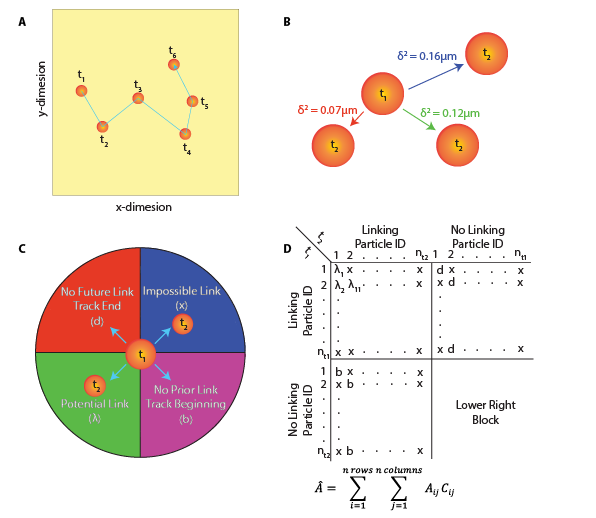
\includegraphics[width=\textwidth]{Figures/"1) Introduction"/SPT-01.png}}
	\caption{Use of a Linear Assignment Problem (LAP) Cost Matrix to Link Particles Between Frames. \textbf{A} Schematic of how a particles trajectory through 		time in an x,y plane may look, $t_n$ refers to the time or frame number. \textbf{B} A particle in $t_1$ will have multiple potential linking particles in $t_2$, 			with an associated cost value $\delta^2$. \textbf{C} The possible outcomes for a particle in $t_2$ following $t_1$. \textbf{D} Schematic of the cost matrix 			utilised in the LAP. To satisfy the LAP, the sum of the cost is minimised as low as possible.}
	\end{figure}

\subsection{Mean squared displacement and diffusion coefficients}

\section{Using SPA}

\subsection{Installing and running SPA}

\subsection{Preparation of image sequences}

\subsection{File directory structure}

\subsection{Setting analysis parameters}

\subsection{Setting threshold values}

\subsection{Running analysis and analysing results}

\end{document}
